\documentclass[letterpaper]{article} % DO NOT CHANGE THIS
\usepackage[submission]{aaai2027}  % DO NOT CHANGE THIS
\usepackage[hyphens]{url}  % DO NOT CHANGE THIS
\usepackage{graphicx} % DO NOT CHANGE THIS
\urlstyle{rm} % DO NOT CHANGE THIS
\def\UrlFont{\rm}  % DO NOT CHANGE THIS
\usepackage{natbib}  % DO NOT CHANGE THIS AND DO NOT ADD ANY OPTIONS TO IT
\usepackage{caption} % DO NOT CHANGE THIS AND DO NOT ADD ANY OPTIONS TO IT
\frenchspacing  % DO NOT CHANGE THIS
\usepackage{booktabs}
\pdfinfo{
/TemplateVersion (2027.1)
}
%%MACROS%%
\setcounter{secnumdepth}{1}

\title{A Held-Out Score Does Not Validate a Glucose Twin's Parameters}
\author{
    Anonymous Submission
}
\affiliations{
}

\begin{document}

\maketitle

\begin{abstract}
A personal glucose twin can show a person a fitted physiological parameter, and a good score on held-out meals is a natural reason to allow that. We test whether such a score supports the claim. We fit a Bergman-type glucose simulator to meals recorded with continuous glucose monitors, and to simulated replicas whose true parameters are known. When the target is the incremental area under the glucose curve (iAUC), no profile-likelihood interval for gastric emptying or carbohydrate absorption is bounded. Held-out iAUC does not show this: on simulated subjects, fits with both rates pinned to wrong extremes have median errors \resNegZeroSlowRefitIauc{} and \resNegZeroFastRefitIauc{} times that of the true model. With exact inputs, the full glucose trace recovers the summed transit time of the two rates, and its 95\% intervals contain the truth in \wsRandAZeroCover{} of \wsN{} simulated subjects. When the logged carbohydrate has a coefficient of variation of 0.75, only \wsRandAThreeQuarterCover{} of \wsN{} contain it, because the estimates shift while the intervals do not widen. Under the same error the number of bounded intervals can rise or fall, depending on where the truths lie. We list the evidence to collect before a fitted parameter is shown as a measurement.
\end{abstract}

\section{Introduction}

An evaluation score supports some claims and not others. Consider an application that tells a person their gastric emptying is slow. A natural piece of evidence for releasing it is that the underlying model predicts meals it has not seen. That score constrains whatever combination of parameters drives the prediction. It need not constrain each parameter, because an optimizer returns a value for every parameter whether or not the data determine it.

The system here is a mechanistic simulator fitted to one person's meals, not an agent. The case is useful because the gap between score and claim can be measured: in simulated replicas the true parameters are known, so each piece of evidence can be compared with what it is taken to show. A closely related study calibrates personal glucose models on oral glucose tolerance tests with continuous glucose monitoring and plasma insulin, and reports better practical identifiability with monitored than with venous glucose \citep{erdos2024leveraging}. Our meals are free-living and self-logged, we have no insulin measurement, and we test each interval on simulations whose parameters we know.

Our contributions are the following.
\begin{enumerate}
\item The iAUC does not determine the two gut rates, and held-out iAUC does not reveal it. Fits with badly wrong rates predict the held-out area almost as well as the true model does.
\item The full trace can recover a combination of the rates when the inputs are exact. Error in the logged carbohydrate moves the estimate without widening its interval.
\item A count of bounded intervals can rise or fall under the same input error, so it does not show that the intervals can be believed. We list evidence that bears on that question.
\end{enumerate}

\section{Related Work}

Identifiability is structural when asked of noise-free output and practical when asked of finite, noisy data \citep{cobelli1980parameter,miao2011identifiability,wieland2021structural}. The profile likelihood diagnoses both \citep{raue2009structural}, and fitted biological models often constrain only combinations of their parameters \citep{gutenkunst2007universally,eisenberg2014determining}. In oral pharmacokinetics, flip-flop kinetics hides which of two serial rates is the slower \citep{boxenbaum1998flipflop}. Models of postprandial response are often evaluated by how well they predict it \citep{zeevi2015personalized,berry2020human}. Our question arises when a mechanistic model's parameters are also reported as quantities about a person.

\section{Setting}\label{sec:setting}

\paragraph{Data.} We use CGMacros \citep{das2025cgmacros}, with \resCohortCgmSubjects{} subjects who logged at least ten meals.

\paragraph{Model.} Each meal is simulated alone from an empty gut with a Bergman-type model \citep{bergman1979} and a two-compartment gut \citep[for a fuller meal model, see][]{dallaman2007}:
\begin{eqnarray}
\dot Q_1 &=& -k_e Q_1 + m(t),\quad \dot Q_2 = k_e Q_1 - k_a Q_2,\nonumber\\
\dot G &=& -(p_1 + X)\,G + p_1 G_b + k_a Q_2 / V_g,\nonumber\\
\dot I &=& -n\,(I - I_b) + \gamma\,[G - G_b]_+,\nonumber\\
\dot X &=& -p_2 X + p_3 S_I\,(I - I_b),\nonumber
\end{eqnarray}
where $Q_1$ and $Q_2$ are stomach and intestinal glucose, $G$ is plasma glucose, $I$ is plasma insulin, $X$ is remote insulin action, $m(t)$ delivers the meal's glucose as a two-minute pulse, and $V_g$ is a distribution volume proportional to body weight. Three parameters are personal: insulin sensitivity $S_I$, gastric emptying rate $k_e$, and carbohydrate absorption rate $k_a$, each confined to a box ($[0.3,1.6]$, $[0.015,0.04]$, and $[0.012,0.032]$ per minute). The remaining constants are fixed at population values.

\paragraph{Targets and estimation.} With $y(t)$ the glucose excursion above the pre-meal mean, set to zero where negative, the iAUC is $\int_0^T y\,dt$ over $T=180$ minutes, and the trace is $y$ at the sampling times. Residuals are Gaussian with a variance per subject and target, estimated at a first fit and then held fixed. Trace residuals are whitened for first-order autocorrelation. Estimates for the profile analyses are refined by L-BFGS-B from several starting points. For the trace we fit $S_I$ and the two combinations $\tau_1=1/k_e+1/k_a$, the summed transit time, and $p=1/(k_e k_a)$, which do not change when the two rates are exchanged. Each point of a $29$-point profile grid is solved to convergence; where the line search fails, it is solved again from two other starting points.

\paragraph{Intervals.} A 95\% profile interval holds the values whose profile negative log-likelihood is within \resDeltaThreshold{} of its minimum \citep{raue2009structural}. It is \emph{bounded} if the likelihood closes it on both sides inside the box. It \emph{covers} the truth if, clipped to the box, it contains the true value. An estimate is \emph{interior} if it lies more than 1\% of the box from both edges. A bounded interval says the likelihood closes, not that the value is right.

\paragraph{Replicas.} A replica simulates each subject's real meals from known true parameters and adds autoregressive sensor noise matched to the subject's residuals. We use truths drawn at random through the box, with two seeds, and truths set to each subject's fitted values. Input error multiplies each logged carbohydrate by lognormal noise with unit mean and a stated coefficient of variation (CV); the data are generated from the true load.

\paragraph{Held-out prediction.} We use five repeats of five-fold cross-validation within subject. On replicas, we divide each fit's held-out error by the error of the model with the true parameters. This reference is not a lower bound, because a fit can absorb input error through $S_I$.

\section{The Area Does Not Determine the Gut Rates}\label{sec:area}

An area keeps little of how a meal arrives \citep{yamaoka1978statistical,cutler1978theory}. Its long-window value depends on the mass delivered and not on the two rates, and at three hours the rates enter mainly through how much has arrived by the end of the window. The Fisher information agrees: under the iAUC its median eigenvalues are \resEigMedianOne{}, \resEigMedianTwo{}, and \resEigMedianThree{}, so one direction is nearly flat.

Table~\ref{tab:box} counts bounded profile intervals under the iAUC. No interval for $k_e$ or $k_a$ is bounded in boxes \wsBoxRange{}. In the primary box most rate estimates lie on a wall, where no interval can close, which is why the wider boxes are the more informative rows. Insulin sensitivity is bounded for some subjects, and how many depends strongly on the box. Whether a displayed sensitivity has a closed interval therefore depends on a search range that the user never sees.

\begin{table}[t]
\centering
\small
\begin{tabular}{lcccccc}
\toprule
 & \multicolumn{2}{c}{$k_e$} & \multicolumn{2}{c}{$k_a$} & \multicolumn{2}{c}{$S_I$} \\
box & int. & bd. & int. & bd. & int. & bd. \\
\midrule
\wsBoxRows
\bottomrule
\end{tabular}
\caption{Subjects (of \wsN{}) with an interior estimate (int.) and with a bounded 95\% interval (bd.) under the iAUC, by box width. No gut rate is bounded; the count for $S_I$ changes with the box.}
\label{tab:box}
\end{table}

\section{What the Held-Out Score Misses}\label{sec:prediction}

On the real data the twin is a modest predictor. Its held-out iAUC error is \resGainPct\% below that of the subject's own mean, and it is worse than that mean on peak time (\resPeakGradThree{} versus \resPeakPersonalMean{} minutes) and on the trace (\resTraceRmseGradThree{} versus \resTraceRmsePersonalMean{} mg\,dL$^{-1}$). Real data also cannot say what the small differences hide, because the true parameters are unknown.

Replicas can. With random truths, the three-parameter fit has a median held-out iAUC error \resPvpRandomZeroRatio{} times that of the true model, although its median root mean square log error in the rates is \resPvpRandomZeroTiming{} (seed 0). To see how much timing error the iAUC can hide, we pinned $(k_e,k_a)$ to the slowest and to the fastest corner of the box and refitted only $S_I$ on each training fold. The median ratios are \resNegZeroSlowRefitIauc{} and \resNegZeroFastRefitIauc{}. A twin whose gut is wrong in either direction therefore looks as good as the fitted one on the target it is evaluated on.

A target the fit did not use sees part of the error. For peak time, the median ratios are \resFloorPeakRandomZeroThreeRatio{} for the fit and \resNegZeroSlowRefitPeak{} and \resNegZeroFastRefitPeak{} for the slow and fast corners. Across subjects, the iAUC ratio of the fit is only weakly related to its rate error (Spearman $\rho$ \figPvpRhoIauc{}, two seeds pooled), whereas the ratios for peak time (\figPvpRhoPeak{}) and for the trace (\figPvpRhoTrace{}) rise with it (Figure~\ref{fig:prediction}). The trace ratio, however, does not separate the corners from the fit in the median, and none of these checks is available on real data, where the true model's error is unknown.

\begin{figure*}[t]
\centering
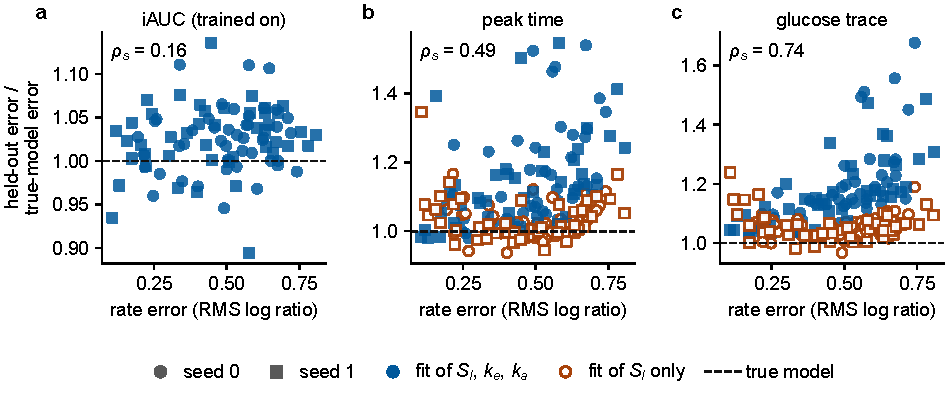
\includegraphics[width=0.93\textwidth]{figures/fig_prediction}
\caption{Held-out error divided by the true model's error, against the error of the two rates, on random-truth replicas (two seeds); all fits use the iAUC. \textbf{(a)} iAUC, \textbf{(b)} peak time, \textbf{(c)} glucose trace. Filled marks: fit of $S_I$, $k_e$, and $k_a$; hollow marks: $S_I$ alone with population rates. $\rho_s$: Spearman correlation for the three-parameter fit. The dashed line is the true model.}
\label{fig:prediction}
\end{figure*}

\section{The Trace, Until the Carbohydrate Log Is Wrong}\label{sec:trace}

The trace carries more timing information than the area. On real CGMacros traces, the interval for $\tau_1$ is bounded in \wsRealTauBd{} of \wsRealTauInt{} interior subjects and the interval for $p$ in \wsRealPBd{} of \wsRealPInt{}. Only simulations can say whether those intervals are right.

\paragraph{Exact inputs.} With exact carbohydrate and the subjects' own sensor noise, the $\tau_1$ interval covers the truth in \wsRandAZeroCover{} of \wsN{} subjects on random-truth seed 0 (seed 1: \wsRandBZeroCover), and the $p$ interval in \wsRandAZeroCoverP{} (seed 1: \wsRandBZeroCoverP). Many intervals are also informative: \wsRandAZeroNarrow{} of the seed-0 $\tau_1$ intervals are bounded and narrower than a factor of about 1.65, and \wsRandAZeroNarrowCover{} of those cover. This is a best case, because the fitted model is the one that generated the data.

\paragraph{Logging error.} As the CV of the logging error grows, coverage falls on all three truth sets (Table~\ref{tab:sweep}); on random-truth seed 0 it goes from \wsRandAZeroCover{} of \wsN{} with exact inputs to \wsRandAThreeQuarterCover{} of \wsN{} at a CV of 0.75. The estimate of $\tau_1$ moves toward slower absorption: on seed 0 the median signed log error grows from \wsRandAZeroShift{} with exact inputs to \wsRandAThreeQuarterShift{} at a CV of 0.75. The median interval width does not grow (\wsRandAZeroWidth{} and \wsRandAThreeQuarterWidth{} in log units). The likelihood treats the logged load as exact, so its interval has no term for doubt about the input. We have not established why the shift is toward slower absorption.

\begin{table}[t]
\centering
\small
\begin{tabular}{llcccc}
\toprule
truths & CV & covers & bounded & shift & rank $\rho$ \\
\midrule
random 0 & 0 & \wsRandAZeroCover & \wsRandAZeroBounded & \wsRandAZeroShift & \wsRandAZeroRho \\
 & 0.25 & \wsRandAQuarterCover & \wsRandAQuarterBounded & \wsRandAQuarterShift & \wsRandAQuarterRho \\
 & 0.75 & \wsRandAThreeQuarterCover & \wsRandAThreeQuarterBounded & \wsRandAThreeQuarterShift & \wsRandAThreeQuarterRho \\
random 1 & 0 & \wsRandBZeroCover & \wsRandBZeroBounded & \wsRandBZeroShift & \wsRandBZeroRho \\
 & 0.25 & \wsRandBQuarterCover & \wsRandBQuarterBounded & \wsRandBQuarterShift & \wsRandBQuarterRho \\
 & 0.75 & \wsRandBThreeQuarterCover & \wsRandBThreeQuarterBounded & \wsRandBThreeQuarterShift & \wsRandBThreeQuarterRho \\
fitted & 0 & \wsFitZeroCover & \wsFitZeroBounded & \wsFitZeroShift & \wsFitZeroRho \\
 & 0.25 & \wsFitQuarterCover & \wsFitQuarterBounded & \wsFitQuarterShift & \wsFitQuarterRho \\
 & 0.75 & \wsFitThreeQuarterCover & \wsFitThreeQuarterBounded & \wsFitThreeQuarterShift & \wsFitThreeQuarterRho \\
\bottomrule
\end{tabular}
\caption{The summed transit time $\tau_1$ on replicas of \wsN{} subjects: intervals covering the truth, bounded intervals, median signed log error of the estimate, and rank correlation between estimates and truths. Coverage falls as the logging error grows.}
\label{tab:sweep}
\end{table}

\paragraph{Bounded counts can mislead.} With random truths, the number of bounded $\tau_1$ intervals falls from \wsRandAZeroBounded{} with exact inputs to \wsRandAThreeQuarterBounded{} at a CV of 0.75 (seed 0). With fitted truths it rises from \wsFitZeroBounded{} to \wsFitQuarterBounded{} between exact inputs and a CV of 0.25. The fitted truths sit near the lower edge of the box (median \wsFitPosPct\% of its width above it; random truths, \wsRandPosPct\%), where many intervals are open below when inputs are exact. A shift toward larger $\tau_1$ moves those estimates away from the edge and closes the intervals, while for truths in the middle of the box it pushes estimates toward the upper edge. A developer who saw more bounded intervals could read worse inputs as better data. An evaluation with truths only at the fitted values would have shown just the rising count.

\paragraph{Ordering.} The ranking of subjects holds up better than coverage: on seed 0 the rank correlation is \wsRandAZeroRho{} with exact inputs and \wsRandAThreeQuarterRho{} at a CV of 0.75. This holds in simulation under the assumed error; real data cannot test it.

\section{Evidence the Claim Needs}\label{sec:checks}

The claim to be supported is that a displayed number measures the named physiological quantity in this person. Our results suggest four pieces of evidence to collect before making it. Each needs only the simulator and the meal records.
\begin{enumerate}
\item State which quantity is shown, what was held fixed to estimate it, and its profile interval with the box that defines it.
\item Score a held-out target that the fit did not use, and do not read accuracy on the training target as support for each parameter.
\item Simulate replicas with the expected input error and with truths spread through the box as well as at the fitted values, and report coverage and interval width, not only the number of bounded intervals.
\item Where only an ordering of people survives those replicas, present an ordering, if anything, and not a physiological value.
\end{enumerate}
More generally, accuracy on the next observation measures prediction. In this case, a claim about a latent quantity needed a test in which that quantity was known.

\section{Limitations}

\paragraph{One model family.} All results are for one Bergman-type simulator with fixed constants, a fixed basal glucose, and no sensor lag. We did not test whether a different gut model changes them.

\paragraph{Assumed input error.} The logging error is independent lognormal noise with unit mean, and its CV is assumed, not measured in these cohorts. We did not test a method that models input error.

\paragraph{Replica design.} Replicas reuse the \wsN{} CGMacros meal schedules, use at most two seeds per truth set, and start each meal from an empty gut, although the median gap between logged meals is \resOverlapMedianGap{} hours and \resOverlapWithinFour\% of gaps are under four hours.

\paragraph{Scope.} All results are for one small cohort. We measured no human outcome, did not study how an unreliable parameter affects the person who sees it, and did not test whether these findings carry over to the evaluation of AI agents.

\section*{Ethical Statement}

All data are public and de-identified, and we collected none. The simulator is a research model that has not been validated for clinical use, and nothing here should inform a medical decision.

\paragraph{Use of generative AI.} We used a large-language-model coding assistant (Claude Code, Anthropic) to write and run analysis code, to generate the scripts that insert stored results into the text and figures, and to draft and edit the manuscript. The authors directed the research and take full responsibility for the content, including its claims and references.

\bibliography{refs}

\end{document}
